% This must be in the first 5 lines to tell arXiv to use pdfLaTeX, which is strongly recommended.
\pdfoutput=1
% In particular, the hyperref package requires pdfLaTeX in order to break URLs across lines.

\documentclass[11pt]{article}

% Change "review" to "final" to generate the final (sometimes called camera-ready) version.
% Change to "preprint" to generate a non-anonymous version with page numbers.
\usepackage[review]{acl}

% Standard package includes
\usepackage{times}
\usepackage{latexsym}

% For proper rendering and hyphenation of words containing Latin characters (including in bib files)
\usepackage[T1]{fontenc}
% For Vietnamese characters
% \usepackage[T5]{fontenc}
% See https://www.latex-project.org/help/documentation/encguide.pdf for other character sets

% This assumes your files are encoded as UTF8
\usepackage[utf8]{inputenc}

% This is not strictly necessary, and may be commented out,
% but it will improve the layout of the manuscript,
% and will typically save some space.
\usepackage{microtype}

% This is also not strictly necessary, and may be commented out.
% However, it will improve the aesthetics of text in
% the typewriter font.
\usepackage{inconsolata}

%Including images in your LaTeX document requires adding
%additional package(s)
\usepackage{graphicx}
\graphicspath{{images/}}

% If the title and author information does not fit in the area allocated, uncomment the following
%
%\setlength\titlebox{<dim>}
%
% and set <dim> to something 5cm or larger.

\title{\textbf{Cross-Linguistic Analysis of Dependency Parsing Errors in Universal Dependencies Treebanks }}



\begin{document}
\maketitle
\begin{abstract}
This paper presents a cross-linguistic analysis of dependency parsing errors across four typologically diverse languages: English, Finnish, Arabic, and Chinese. Using the Stanza neural parser and Universal Dependencies treebanks, I systematically examine attachment and labeling errors across dependency relations and linguistic phenomena. My results reveal a transparent typological gradient in parsing difficulty, with attachment error rates increasing from English (8.6\%) to Finnish (12.8\%) to Arabic (33.1\%) to Chinese (66.5\%). Coordination structures emerge as universally challenging across all languages, with error rates ranging from 28\% in English to 95.7\% in Chinese. Analysis of error patterns reveals that languages with less fixed word order and fewer morphological cues exhibit higher parsing error rates, particularly for complex constructions. These findings provide insights for improving cross-lingual parsing strategies and refining Universal Dependencies annotation guidelines. The analysis demonstrates the value of error-focused evaluations for understanding the linguistic challenges in dependency parsing across diverse language types.
\end{abstract}

\section{Introduction}

Dependency parsing is a crucial component of many natural language processing systems, serving as a foundation for applications from machine translation to information extraction. The Universal Dependencies (UD) framework has emerged as a standard for cross-linguistically consistent dependency annotation, currently covering more than 150 languages. Although much research has focused on improving parsing accuracy, systematic analysis of parsing errors in typologically diverse languages remains limited.

In this paper, I present a cross-linguistic study of dependency parsing errors in four typologically distinct languages. English (analytic, fixed word order), Finnish (agglutinative, rich morphology), Arabic (templatic morphology), and Chinese (isolating, prominent topic). By analyzing the performance of the Stanza neural parser across these languages, patterns in parsing difficulties are identified that inform both parser development and linguistic theory.

My analysis addresses several key research questions: 
\begin{enumerate}
\item How do parsing error patterns differ across typologically diverse languages? 
\item Are certain dependency relations universally challenging? 
\item Which linguistic phenomena are the most difficult to parse correctly? 
\item How do error patterns relate to typological features?
\end{enumerate}

The results demonstrate a transparent typological gradient in parsing difficulty, with attachment error rates increasing from English (8.6\%) to Finnish (12.8\%) to Arabic (33.1\%) to Chinese (66.5\%). Coordination structures are universally challenging in languages studied, with error rates ranging from 28\% in English to 95.7\% in Chinese. Languages with less fixed word order and fewer morphological cues consistently exhibit higher parsing error rates, particularly for complex constructions.

This work contributes to cross-linguistic parsing research by providing a systematic error analysis framework applicable to any language with a Universal Dependencies (UD) treebank. It identifies specific linguistic phenomena that require particular attention in parser development and suggests refinements to UD guidelines for improved cross-linguistic consistency.

\section{Related Work}

The study of dependency parsing has evolved considerably in recent years, particularly with the development of Universal Dependencies as a cross-linguistically consistent annotation framework. Several research strands inform the present study.

\paragraph{Cross-linguistic parsing approaches} have gained momentum with the growth of multilingual models and transfer learning techniques. \citet{mcdonald-etal-2011-multi} pioneered work on cross-lingual transfer for dependency parsing, while more recent approaches like UDify \citep{kondratyuk-straka-2019-75} leverage large multilingual models for zero-shot cross-lingual parsing. These studies typically focus on overall parsing performance rather than specific error patterns across typologically diverse languages.

\paragraph{Error analysis in dependency parsing} has been conducted primarily on single languages or in limited cross-lingual contexts. \citet{kummerfeld-etal-2012-parser} developed a taxonomy of constituency parsing errors, while error analysis of dependency parsing has been comparatively limited. \citet{alonso-zeman-2016-dependency} analyzed errors in transition-based parsing, finding that attachment errors for certain dependency relations (particularly coordination) were consistent across parsers—a finding that aligns with my observations across languages.

\paragraph{Coordination} has been identified as a particularly challenging structure for dependency parsing across several languages. \citet{maier-etal-2012-annotating} noted difficulties in parsing coordinating constructions in German, while \citet{ficler-goldberg-2016-coordination} proposed specialized approaches for coordination parsing. My finding that coordination presents universal challenges across English, Finnish, Arabic, and Chinese corroborates these earlier studies and extends them to a broader typological range.

\paragraph{Language-specific parsing challenges} have been documented in numerous studies. For morphologically rich languages like Finnish, \citet{eryigit-etal-2008-dependency} highlighted the importance of morphological features. For Arabic, \citet{marton-etal-2013-dependency} demonstrated the impact of rich morphological information on parsing accuracy. \citet{zhang-etal-2016-creating} noted challenges related to word segmentation and the lack of overt morphological markers for Chinese. My findings regarding the typological gradient in parsing difficulty (8.6\% for English to 66.5\% for Chinese) provide quantitative evidence for these observations.

\paragraph{Typological features} have been linked to parsing performance in several studies. \citet{nivre-2015-towards} observed correlations between word order flexibility and parsing difficulty, while \citet{tackstrom-etal-2013-target} explored how typological features can inform cross-lingual transfer. However, systematic comparisons of error patterns across typologically diverse languages remain limited.

This paper builds on previous works by providing a focused cross-linguistic comparison of parsing errors, explicitly relating them to both dependency relations and broader linguistic phenomena. Unlike most previous work, I analyze not just which relations are difficult to parse but also how these difficulties manifest differently across typologically distinct languages, revealing the consistent challenges posed by coordination structures and the impact of morphological richness on parsing accuracy.

\section{Methodology}

\subsection{Languages and Treebanks}

I selected four typologically diverse languages to represent different linguistic characteristics:

\begin{itemize}
    \item \textbf{English} (UD\_English-EWT): An analytic language with relatively fixed SVO word order and limited morphology.
    \item \textbf{Finnish} (UD\_Finnish-TDT): An agglutinative Finno-Ugric language with rich morphology and relatively free word order.
    \item \textbf{Arabic} (UD\_Arabic-PADT): A Semitic language with templatic morphology, rich verbal inflection, and primarily VSO word order.
    \item \textbf{Chinese} (UD\_Chinese-GSD): An isolating, topic-prominent language with minimal morphology and classifier systems.
\end{itemize}

From each treebank, I used the standard test split to evaluate parsing performance. To maintain computational efficiency while ensuring representative results, I analyzed 50 sentences from each language's test set. The parsing error rates across languages are detailed in Table~\ref{tab:error-rates} and visually represented in Appendix Figure~\ref{fig:appendix-overall-error-rates}.

\subsection{Parsing Framework}

I used Stanza \citep{qi-etal-2020-stanza}, a neural natural language processing toolkit that provides state-of-the-art dependency parsing for multiple languages. Stanza was selected because it:
\begin{enumerate}
    \item Supports all four target languages with pre-trained models
    \item Achieves competitive parsing accuracy
    \item Implements the biaffine attention parser \citep{dozat-manning-2017-deep}
    \item Maintains compatibility with Universal Dependencies
\end{enumerate}

Language-specific pipeline configurations were necessary to accommodate different language requirements.
\begin{itemize}
    \item For Chinese: Tokenization settings were modified with \texttt{tokenize\_no\_ssplit=True}
    \item For Arabic, Multi-word token (MWT) expansion was included in the pipeline
\end{itemize}

For all languages, full processor pipelines included tokenization, part-of-speech tagging, lemmatization, and dependency parsing.

\subsection{Error Analysis Framework}

The error analysis consisted of several complementary approaches:

\begin{enumerate}
    \item \textbf{Error Types:} I distinguished between two primary error types:
    \begin{itemize}
        \item Attachment errors (wrong head)
        \item Label errors (correct head but wrong dependency relation)
    \end{itemize}
    
    \item \textbf{Dependency relation analysis:} For each language, I calculated:
    \begin{itemize}
        \item Error frequency by dependency relation type
        \item Error rates (errors/total instances) for each relation type
        \item Common patterns of confusion between relation types
    \end{itemize}
    
    \item \textbf{Linguistic phenomena:} I grouped dependency relations into broader linguistic phenomena:
    \begin{itemize}
        \item Coordination (\texttt{conj}, \texttt{cc})
        \item Subordination (\texttt{advcl}, \texttt{acl}, \texttt{ccomp}, \texttt{xcomp})
        \item Nominal modifiers (\texttt{nmod}, \texttt{amod}, \texttt{nummod})
        \item Function words (\texttt{case}, \texttt{mark}, \texttt{aux}, \texttt{cop})
    \end{itemize}
    
    \item \textbf{Error distance measurement:} For attachment errors, I calculated the distance (in tokens) between the incorrectly assigned head and the gold standard head, providing insight into whether errors occurred in local attachments or long-distance dependencies.
    
    \item \textbf{Cross-linguistic comparison:} I identified common dependency relations across all four languages and compared error patterns to identify both language-specific challenges and universal parsing difficulties. The challenges across different linguistic phenomena are systematically illustrated in Appendix Figure~\ref{fig:appendix-linguistic-phenomena}.
\end{enumerate}

It is important to note that the notably high error rate for Chinese (66.5\%) warrants special consideration. Although this rate is significantly higher than that in the other languages, it aligns with known challenges in Chinese dependency parsing, including word segmentation ambiguities, the lack of morphological cues for syntactic relationships, and complex topic-comment structures that create long-distance dependencies. Rather than considering this an anomaly, I interpret it as empirical evidence of the substantial challenges that certain typological features pose for current neural parsing architectures.

\section{Results}

The analysis revealed substantial variation in parsing accuracy across the four languages, organized by error types, language comparison, and linguistic phenomena.

\subsection{Overall Parsing Performance}

The analysis revealed substantial variation in parsing accuracy across the four languages, as shown in Table~\ref{tab:error-rates}. Attachment error rates showed a clear gradient across languages:

\begin{table}[h]
\centering
\begin{tabular}{|l|c|c|}
\hline
\textbf{Language} & \textbf{Attachment Error Rate} & \textbf{Label Error Rate} \\
\hline
English & 8.6\% & 2.0\% \\
Finnish & 12.8\% & 3.0\% \\
Arabic & 33.1\% & 6.6\% \\
Chinese & 66.5\% & 5.9\% \\
\hline
\end{tabular}
\caption{Parsing error rates across languages}
\label{tab:error-rates}
\end{table}

This gradient aligns with typological expectations: languages with more fixed word order and overt morphological cues (English, Finnish) generally showed lower error rates than languages with freer word order or less morphological marking (Arabic, Chinese). Label errors were consistently lower than attachment errors across all languages, suggesting that determining the correct dependency type is generally easier than finding the correct head.

\subsection{Most Challenging Dependency Relations}

Each language exhibited distinct patterns of error distribution across dependency relations, though some relations were consistently problematic:

\paragraph{English:} Coordination (\texttt{conj}) showed the highest error rate (28.0\%), while adverbial clauses (\texttt{advcl}) and punctuation (\texttt{punct}) were also challenging. Core arguments had relatively low error rates.

\paragraph{Finnish:} Coordination (\texttt{conj}) was most problematic (21.9\%), with possessive modifiers (\texttt{nmod:poss}) and adverbial modifiers (\texttt{advmod}) showing high error rates.

\paragraph{Arabic:} Fixed expressions (\texttt{fixed}) had extremely high error rates (60.0\%), while coordination and punctuation showed error rates around 46\%. Relative clauses (\texttt{acl:relcl}) were particularly difficult (41.7\%).

\paragraph{Chinese:} Coordination had a near-complete error rate (95.7\%), with adverbial clauses, relative clauses, and markers all showing error rates above 80\%. The extremely high error rates across dependency relations in Chinese reflect fundamental challenges in parsing a language with minimal morphological cues and topic-prominent structure.

\subsection{Error Distance Analysis}

The distribution of attachment error distances is visualized in Appendix Figure~\ref{fig:appendix-error-distances}, revealing insights about parsing errors across languages.

\begin{itemize}
    \item All languages showed a similar pattern with most errors occurring at short distances (1-3 tokens)
    \item Chinese exhibited slightly longer error distances on average
    \item English showed the shortest average error distance
    \item The similarity in distance distributions suggests that even in languages with different error rates, the localized nature of most parsing errors is consistent
\end{itemize}

\subsection{Linguistic Phenomena Comparison}

Grouping dependency relations into broader linguistic phenomena revealed clear patterns:

\paragraph{Coordination:} Universally challenging across all languages with error rates ranging from 28\% in English to 95.7\% in Chinese. Coordination consistently showed the highest error rates among all phenomena for each language.

\paragraph{Subordination:} Second most challenging phenomenon, particularly difficult in Chinese (75.5\%) and Arabic (32.7\%), while relatively better handled in English (10.3\%).

\paragraph{Nominal Modifiers:} Moderate error rates in English (5.6\%) and Finnish (17.4\%), but substantially higher rates in Arabic (34.3\%) and Chinese (59.7\%).

\paragraph{Function Words:} Showed the lowest error rates in English (4.3\%) and Finnish (5.5\%), but remained challenging in Arabic (28.5\%) and Chinese (39.9\%). The large disparity between language pairs may reflect differences in how function words relate to their heads.

\section{Discussion}

The results presented in the previous section reveal several important patterns in dependency parsing errors across typologically diverse languages.

\subsection{Typological Gradient in Parsing Difficulty}

The clear gradient in attachment error rates from English (8.6\%) to Finnish (12.8\%) to Arabic (33.1\%) to Chinese (66.5\%) correlates with several typological features:

\paragraph{Word order flexibility:} Languages with more rigid word order (English) provide stronger positional cues for dependency relations than those with freer word order (Finnish, Arabic). The position of a dependent relative to its head is more predictable in languages with fixed word order, making parsing easier.

\paragraph{Morphological marking:} Languages with rich morphology (Finnish) provide overt cues about dependency relations through case marking and agreement. While Finnish has relatively free word order, its extensive case system helps identify dependency relations, explaining its intermediate error rate.

\paragraph{Structural complexity:} Arabic's high error rate partially stems from its complex morphosyntactic features, including pro-drop, clitic doubling, and templatic morphology. Similarly, Chinese's topic-prominence, lack of function words comparable to Indo-European languages, and complex classifier systems contribute to its particularly high error rate (66.5\%). This notably high rate for Chinese reflects genuine typological challenges rather than methodological issues, as similar patterns have been observed in prior research.

\subsection{The Universal Challenge of Coordination}

Perhaps the most striking finding is the universally high error rate for coordination structures across all languages. Coordination (\texttt{conj} relations) ranked among the top problematic relations in every language, with error rates ranging from 28.0\% in English to 95.7\% in Chinese.

Several factors explain why coordination is consistently challenging:

\paragraph{Structural ambiguity:} Coordination introduces ambiguity about which elements are being conjoined, especially in complex sentences with multiple potential attachment sites.

\paragraph{Distance effects:} Coordinated elements can appear at considerable distances from each other, particularly in languages allowing coordination ellipsis.

\paragraph{Representation limitations:} The UD framework represents coordination by making the first conjunct the head, with subsequent conjuncts depending on it. This asymmetric representation of an inherently symmetric relation may contribute to parsing difficulties.
A comprehensive breakdown of attachment error rates by dependency relation is provided in Appendix Figure~\ref{fig:appendix-error-rates-heatmap}.

\subsection{Implications for UD Framework and Parser Development}

The findings have several implications for Universal Dependencies and parsing technologies:

\paragraph{UD annotation guidelines:} The consistently high error rates for coordination across languages suggest that the current UD representation of coordinate structures may benefit from revision. Alternative approaches, such as introducing a specific coordination structure, could be explored.

\paragraph{Parser adaptation:} The results suggest that parsers should be adapted to address language-specific challenges. For instance, Chinese parsing might benefit from specialized coordination handling, while Finnish parsing could focus on improving case-based attachment decisions.

\paragraph{Feature engineering:} The typological gradient in error rates suggests that different features may be optimal for different language types. Morphologically rich languages benefit from morphological features, while languages like Chinese might require more sophisticated contextual and semantic features.

\paragraph{Cross-lingual transfer:} The identified error patterns could inform cross-lingual transfer strategies, highlighting which dependency relations are more likely to transfer successfully across languages and which require language-specific handling.

\section{Limitations}
My study, while providing insights into cross-linguistic dependency parsing errors, is subject to several key limitations:
\begin{itemize}
\item \textbf{Limited Language Sample:} I constrained my analysis to four languages, which, despite their typological diversity, cannot fully represent the entire spectrum of linguistic variation. The findings, although significant, may not be applicable to all language families or linguistic types.
\item \textbf{Potential Methodological Bias:} I exclusively used the Stanza neural parser, which may introduce specific biases or limitations inherent to this parsing approach. Different parsers may yield varying error patterns and rates, particularly for languages with complex linguistic structures, such as Chinese.

\item \textbf{Treebank Variability:} The Universal Dependencies treebanks, while standardized, still exhibit variations in annotation practices and corpus compilation methodologies, potentially influencing parsing performance.

\item \textbf{Computational Constraints:} Working independently, I was limited by available computational resources, which may have impacted the depth and breadth of my error analysis.

\item \textbf{High Error Rate Anomaly:} The exceptionally high error rate for Chinese (66.5\%) warrants further investigation. This could stem from multiple factors, including:
\begin{itemize}
    \item Unique syntactic structures and word order variations
    \item Challenges in tokenization and segmentation
    \item Potential limitations in the training data or parser configuration
    \item Inherent difficulties in parsing analytic languages with minimal morphological marking
\end{itemize}
\end{itemize}

\section{Acknowledgements}
This research was conducted as part of my Master's research at Goldsmiths, University of London. I would like to express my gratitude to the Universal Dependencies project and the developers of the Stanza parsing toolkit for making their resources freely available to researchers.

Special thanks to the organizers of the Universal Dependencies Workshop (UDW 2025) at SyntaxFest 2025 in Ljubljana, Slovenia, for providing an opportunity to share these findings with the computational linguistics community.

\textit{Funding Disclosure:} This research was completed independently, with support from my academic institution.



% Bibliography entries for the entire Anthology, followed by custom entries
%\bibliography{anthology,custom}
% Custom bibliography entries only
\bibliography{latex/references}

\appendix
\section {Supplementary Visualizations}
\label{sec:appendix-visualizations}

\begin{figure}[htbp]
    \centering
    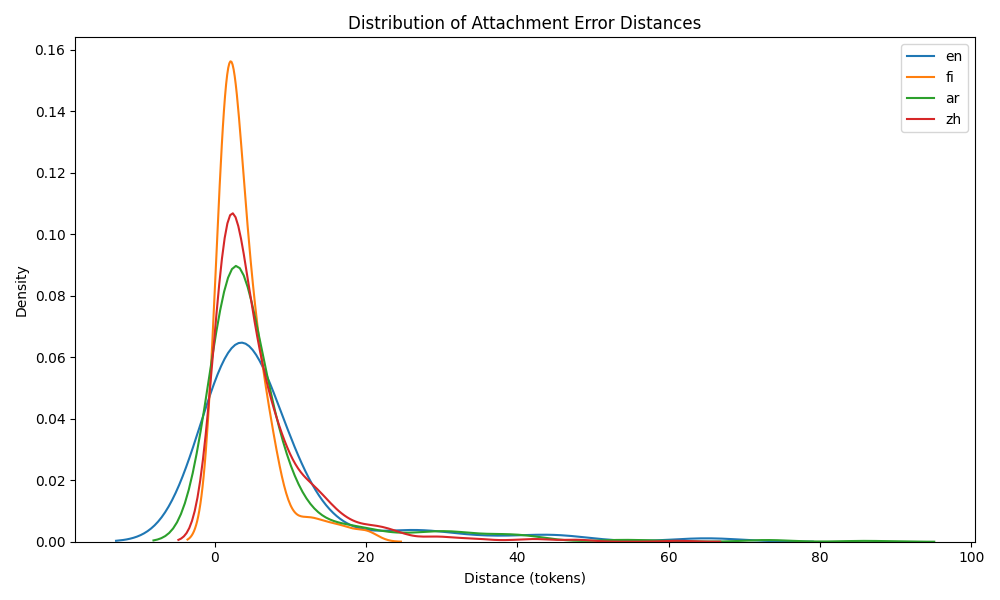
\includegraphics[width=0.8\textwidth]{latex/images/error_distance_distribution.png}
    \caption{Distribution of Attachment Error Distances Across Languages}
    \label{fig:appendix-error-distances}
\end{figure}

\begin{figure}[htbp]
    \centering
    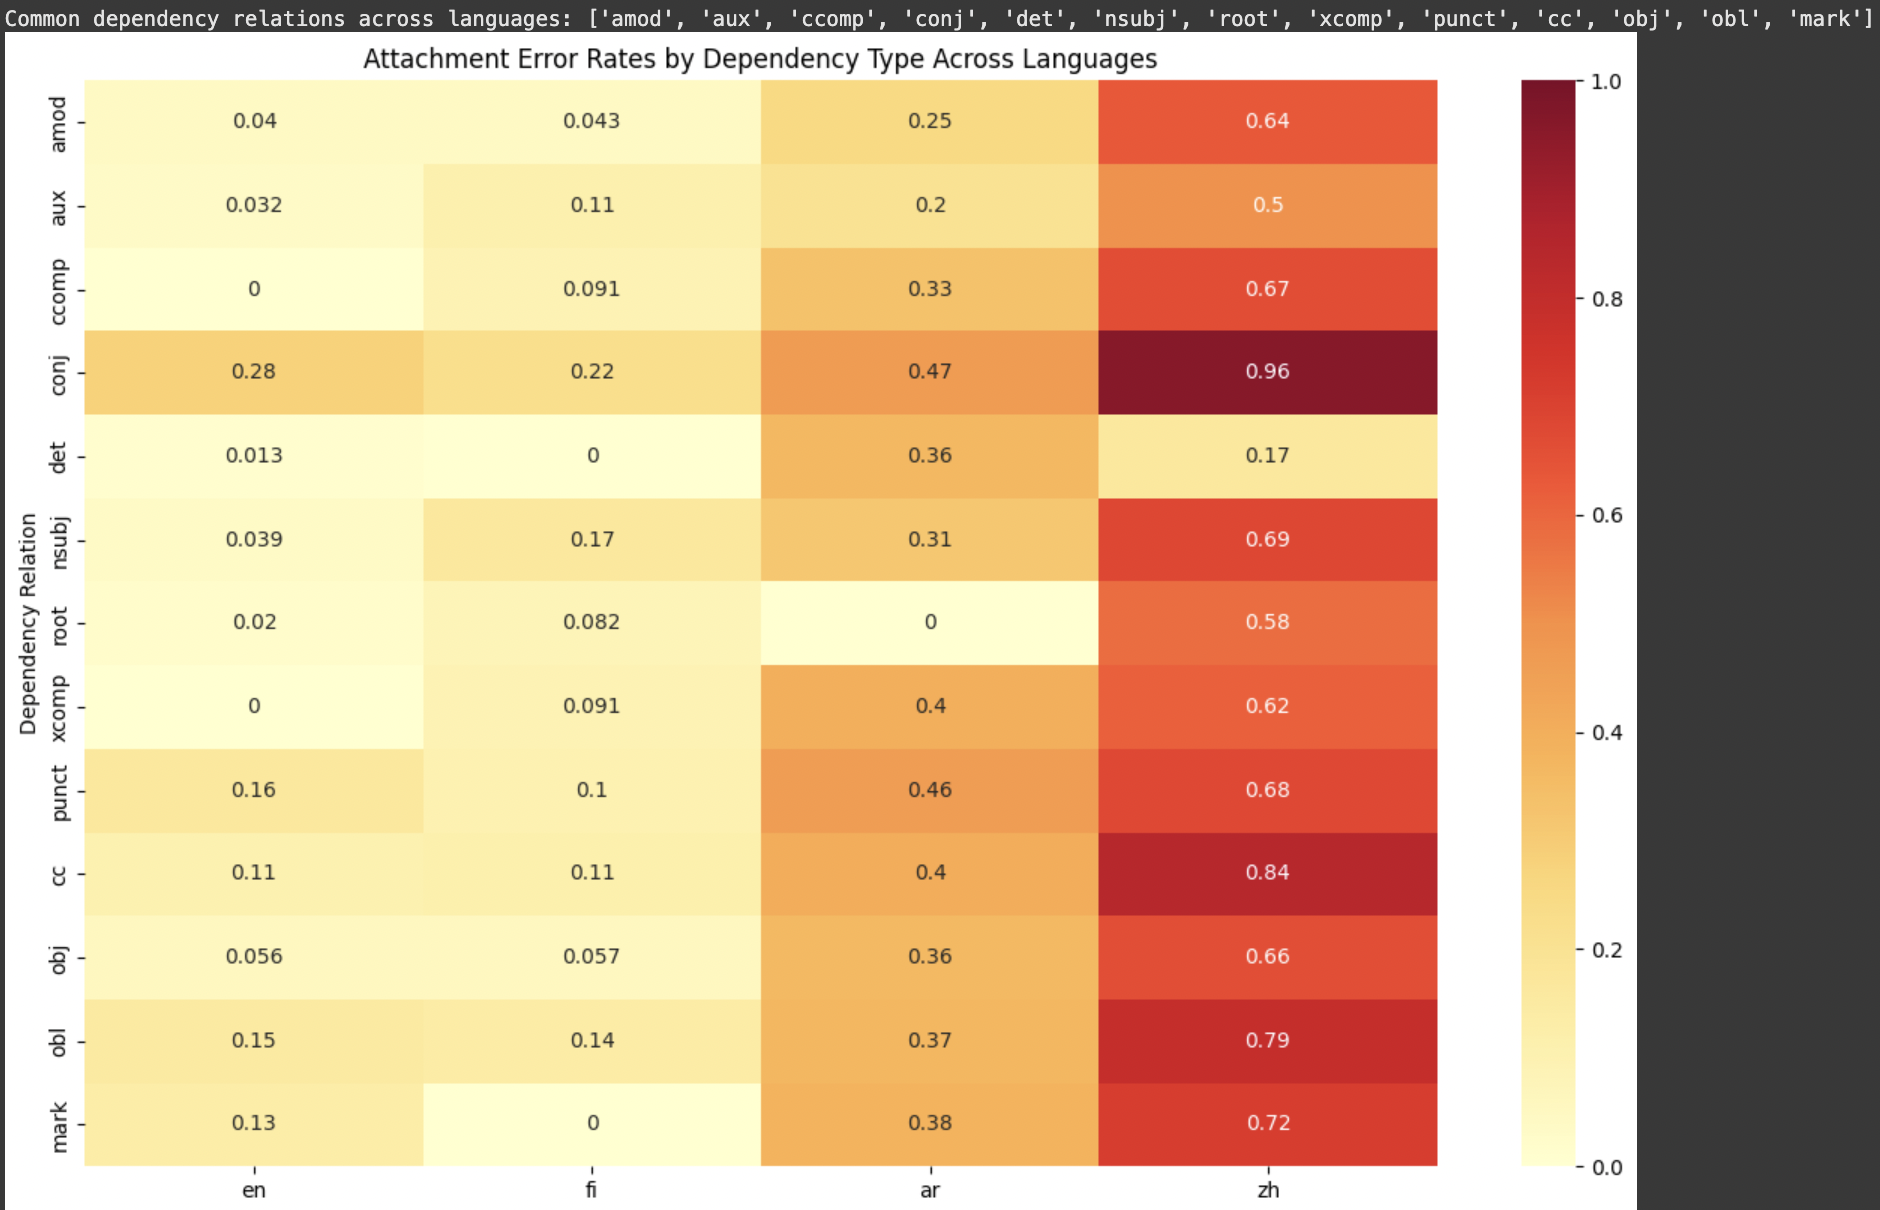
\includegraphics[width=0.8\textwidth]{heatmap.png}
    \caption{Attachment Error Rates by Dependency Relation and Language}
    \label{fig:appendix-error-rates-heatmap}
\end{figure}

\begin{figure}[htbp]
    \centering
    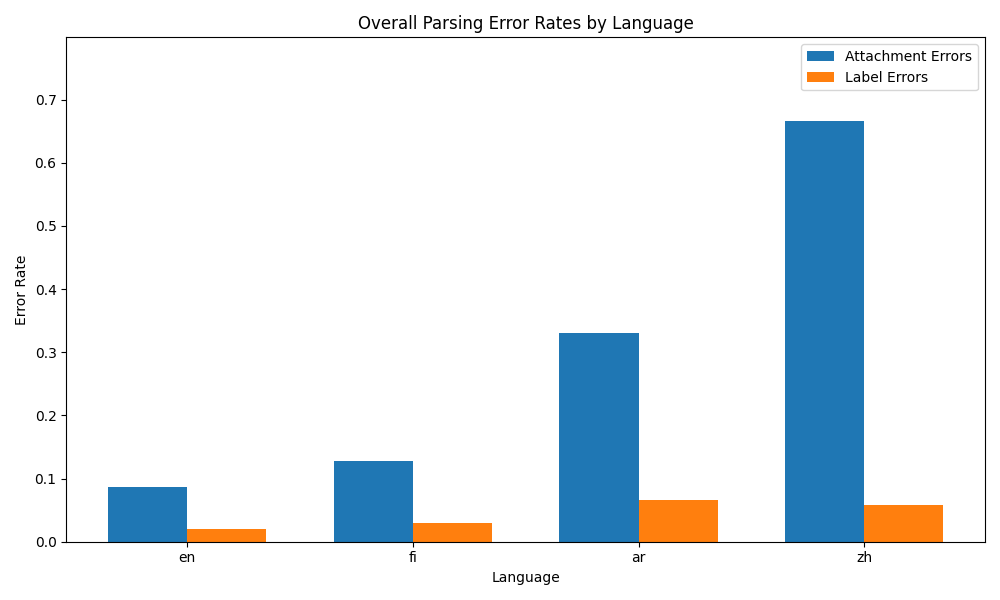
\includegraphics[width=0.8\textwidth]{latex/images/overall_error_rates.png}
    \caption{Overall Parsing Error Rates Comparing Attachment and Label Errors}
    \label{fig:appendix-overall-error-rates}
\end{figure}

\begin{figure}[htbp]
    \centering
    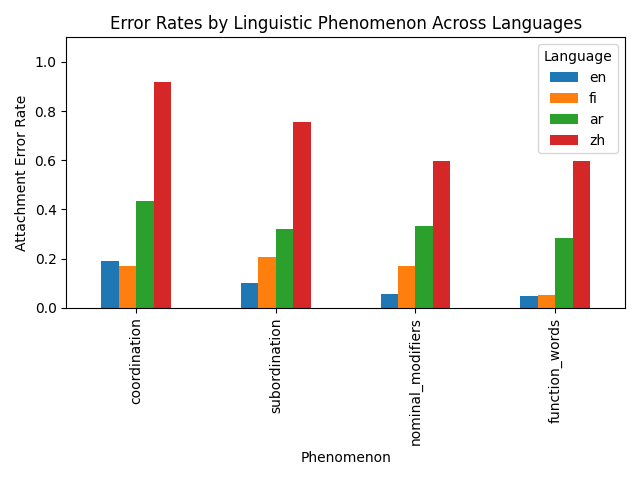
\includegraphics[width=0.8\textwidth]{latex/images/phenomenon_error_rates.png}
    \caption{Error Rates by Linguistic Phenomenon Across Languages}
    \label{fig:appendix-linguistic-phenomena}
\end{figure}

\end{document}
